\chapter{Inverting Configurations}
\section{Inverting Amplifier}

\begin{figure}
	\centering
	\begin{subfigure}{0.4\textwidth}
		\centering
		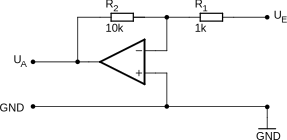
\includegraphics[width=.9\linewidth]{./img/schem-inv.pdf}
		\caption{Basic Inverting Amplifier with Gain 10}
		\label{schem:inv}
	\end{subfigure}
	\begin{subfigure}{0.4\textwidth}
		\centering
		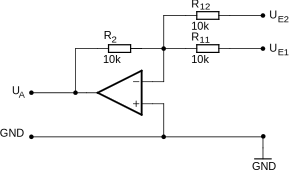
\includegraphics[width=.9\linewidth]{./img/schem-add.pdf}
		\caption{Inverting Adder}
		\label{schem:add}
	\end{subfigure}
\end{figure}

In the inverting configuration shown in \autoref{schem:inv}, the input signal is fed into the feedback loop, the non-inverting input is held at a fixed voltage.
As the opamp is configured for negative feedback, both inputs are held at the same potential which is often ground.
As the inverting input is not directly connected to a voltage source, it's node is called a 'virtual ground'.

Unlike the non-inverting amplifier, the input of the inverting amplifier has a low input impedance, set by \comp{R_1}.

The gain of the circuit is calculated from the current through \comp{R_1} to the virtual ground node: $I_\comp{R_1} = \frac{\ue}{R_1}$, which is equal to the current through \comp{R_2}: $I_\comp{R_2} = \frac{\ua}{R_2}$.
Using a consistent reference direction, the gain  $A$ is \[A = \frac{\ua}{\ue} = -\frac{R_2}{R_1}\].

\section{Inverting Adder}

Ignoring \comp{R_1} in \autoref{schem:inv}, the output voltage \ua is $\ua = -R_2 \cdot I_\text{in}$, with the total current $I_\text{in}$ flowing into the virtual ground node of the inverting input.
As the voltage at this node is independent of $I_\text{in}$, more inputs can be connected, each via a resistor that controls the gain of the respective input.
The individual input currents add up to $I_\text{in}$ and the output voltage is \[\ua = -R_2 \cdot \left(\frac{{\ue}_1}{R_{11}} + \frac{{\ue}_2}{R_{12}} + \dots\right)\] with the component labels shown in \autoref{schem:add}.
